\documentclass[a4paper, 12pt]{extreport}
\usepackage[margin=1in]{geometry}
\usepackage{tikz}
\usetikzlibrary{calc}
\usepackage{setspace}
\graphicspath{ {../../resources/images/} }
\usepackage[titles]{tocloft}
\usepackage{titlesec}
\usepackage[hidelinks]{hyperref}
\usepackage{pdfpages}
\titleformat{\chapter}[hang]{\huge\bfseries}{\thechapter}{20pt}{\vspace{0.5em}}
\titlespacing*{\chapter}{0pt}{-3em}{1.1\parskip}
\usepackage[backend=biber, style=ieee]{biblatex}
\usepackage{parskip}
\setlength{\parindent}{1cm}
\setlength{\parskip}{.5\baselineskip}
\usepackage[nottoc,numbib]{tocbibind}
\addbibresource{../../resources/citation.bib}
\usepackage{tabularx}
\usepackage{multirow}
\usepackage{amsmath}

\begin{document}
	
	% defining pieces for figures
	\def\opiece{\tikz{\draw[fill=yellow](0,0) rectangle (2,2);}}
	\def\ipiece{\tikz{\draw[fill=cyan](0,0) rectangle (4,1);}}
	\def\tpiece{\tikz{\draw[fill=violet](0,0) -- (3,0) -- (3,1) -- (2,1) -- (2,2) -- (1,2) -- (1,1) -- (0, 1) -- cycle;}}
	\def\zpiece{\tikz{\draw[fill=red](0,1) -- (1,1) -- (1,0) -- (3,0) -- (3,1) -- (2,1) -- (2,2) -- (0,2) -- cycle;}}
	\def\spiece{\tikz{\draw[fill=green](0,0) -- (2,0) -- (2,1) -- (3,1) -- (3,2) -- (1,2) -- (1,1) -- (0,1) -- cycle;}}
	\def\jpiece{\tikz{\draw[fill=blue](0,0) -- (3,0) -- (3,1) -- (1,1) -- (1,2) -- (0,2) -- cycle;}}
	\def\lpiece{\tikz{\draw[fill=orange](0,0) -- (3,0) -- (3,2) -- (2,2) -- (2,1) -- (0,1) -- cycle;}}
	\def\garbage#1#2{\tikz{\draw[fill=black!40!white](0,0) -- (0,#1) -- (#2-1,#1) -- (#2-1,0) -- cycle; \draw[fill=black!40!white](#2, 0) -- (10,0) -- (10,#1) -- (#2,#1) -- cycle}}

	\onehalfspacing
	
	\begin{titlepage}
		
		\begin{tikzpicture}[remember picture, overlay]
			\node[xshift=14cm,yshift=-1.8cm,anchor=north west] at (current page.north west){%
				
\includegraphics[height=2.5cm]{logos/sunway}};
		\end{tikzpicture}
		
		\vfill
		
		\begin{center}
			\textbf{\large CAPSTONE PROJECT 1} \\
			\textbf{\large Planning Document} \\
			\vspace{1cm}
			\textbf{\large Evaluation of Nature-inspired Optimisation\\Algorithms in Solving Versus Tetris}
			
			\vspace{1cm}
			
			by
			
			\vspace{1cm}
			
			\large Yap Wei Xiang \\
			21067939
			
			\vspace{1cm}
			
			\large Supervisor: Dr Richard Wong Teck Ken
			
			\vspace{1cm}
			
			\normalsize Semester: April 2024 \\
			Date: % TODO: DATE OF SUBMISSION
			
			\vfill
			
			Department of Computing and Information Systems\\
			School of Engineering and Technology\\
			Sunway University
		\end{center}
		
	\end{titlepage}
	
	\pagenumbering{roman} % switch to roman numerals
	
	\chapter*{Abstract}
	
	\addcontentsline{toc}{chapter}{Abstract}
	
	\tableofcontents
	
	\listoftables
	
	\listoffigures
	
	\chapter{Introduction}
	
		\pagenumbering{arabic}
		
		% What is Tetris		
		Tetris is a popular video game created in 1984 by computer programmer Alexey Pajitnov  \cite{about-tetris}. It is a puzzle game that requires players to strategically place sequences of pieces known as "Tetriminos" into a rectangular Matrix (refer to Figure \ref{fig:tetrisgame}). In the classic game, players attempt to clear as many lines as possible by completely filling horizontal rows of blocks, but if the Tetriminos surpass the top of the Matrix, the game ends.
		
		\begin{figure}[h]
			\centering
				\begin{tikzpicture}[every node/.style={inner sep=-0.4pt,anchor=south west,scale=.4},scale=.4]
					\coordinate (sw) at (5,0);
					\coordinate (nw) at (5,20);
					\coordinate (se) at (15,0);
					\coordinate (ne) at (15,20);
					\draw[fill=black!10!white] (sw) -- (nw) -- (ne) -- (se) -- cycle;
					\node at ($(nw) - (4,5)$){\spiece};	
					\node at (sw){\ipiece};
					\node at ($(sw) + (4,0)$){\opiece};
					\node at ($(sw) + (2,1)$){\spiece};
					\node at ($(sw) + (1,1)$){\rotatebox{90}{\zpiece}};
					\node at ($(sw) + (0,1)$){\rotatebox{-90}{\jpiece}};
					\node at ($(sw) + (6,0)$){\tpiece};
					\node at ($(sw) + (7,1)$){\rotatebox{90}{\lpiece}};
					\node at ($(sw) + (5,1)$){\rotatebox{180}{\tpiece}};
					\node at ($(sw) + (2,3)$){\zpiece};
					\node at ($(sw) + (5,3)$){\opiece};
					\node at ($(se) - (1,-5)$){\rotatebox{90}{\ipiece}};
					\node at ($(ne) + (1,-2)$){\lpiece};
					\node at ($(ne) + (1,-5)$){\jpiece};
					\node at ($(ne) + (1,-8)$){\opiece};
					\node at ($(ne) + (1,-11)$){\ipiece};
					\node at ($(ne) + (1,-14)$){\tpiece};
					\draw[ultra thick] (sw) -- (nw) -- (ne) -- (se) -- cycle;
				\end{tikzpicture}
			\caption{\centering A typical modern Tetris game where four lines are about to be cleared. The Tetrimino on the left of the matrix is the \textit{Hold} piece and the pieces to the right of the matrix are collectively known as the \textit{Queue}.}
			\label{fig:tetrisgame}
		\end{figure}
		
		% Tetris and computer science
		Since its release, mathematicians and computer scientists have been intrigued by the game of Tetris, leading to a diverse array of research endeavours exploring the various facets of the game, including its computational complexity \cite{tetris-is-hard-even-to-approx}, and its possibility of being won \cite{can-you-win-at-tetris} \cite{how-to-lose-at-tetris}.
		
		\section{Motivation}
		
			% In this section, you'll explain why your capstone project is important and relevant. What inspired you to pursue this topic? Is there a particular problem or challenge in the field that you're interested in addressing?
			% Consider discussing the broader significance of your research topic, such as its potential impact on society, industry, or academia. Why should readers care about your project?
			% You might also highlight any personal or professional experiences that motivated your interest in the topic.
	 		
	 		In their paper, \citeauthor{tetris-is-hard-even-to-approx} showed that it is NP-complete to optimise several natural objective functions of Tetris \cite{tetris-is-hard-even-to-approx}. NP-completeness poses a significant challenge in computational problem-solving, as it denotes the absence of polynomial-time algorithms for efficient solutions \cite{sipser-intro-to-computation}. Moreover, the discovery of a polynomial-time algorithm for any NP-complete problem implies that any problem in the set of NP, encompassing efficiently verifiable but potentially difficult problems, could be solved in polynomial time \cite{sipser-intro-to-computation}. NP-completeness extends beyond Tetris, with real-life instances of NP-complete arising in diverse fields such as route optimisation \cite{route-optimisation-np-complete}, job scheduling \cite{job-scheduling-np-complete}, and medicine \cite{medical-diagnosis-np-complete}.
	 		
	 		To address these challenges, researchers have explored alternative approaches to tackle NP-complete problems, including the use of nature-inspired algorithms \cite{job-shop-ga}. Although they might fail at finding optimal solutions, nature-inspired algorithms are able to return acceptable solutions in shorter running times \cite{review-nia-wael}. In the context of optimising Tetris gameplay, studies have shown the effectiveness of using nature-inspired algorithms in playing the classic single-player game \cite{tetris-ga-lewis} \cite{swarm-tetris}. However, there remains limited research on the effectiveness of nature-inspired optimisation algorithms in the multiplayer versus variant of the game.
			
		\section{Problem Statement}
			
			% Here, you'll clearly define the problem or issue that your capstone project aims to address. What specific challenge or question are you seeking to answer?
			% Describe the current state of the problem and any existing solutions or approaches. What limitations or shortcomings do these solutions have?
			% Be concise and specific in articulating the problem statement, making it clear to readers what your project seeks to contribute to the field.
			
			% Despite the extensive research on classic Tetris, there is a significant gap in the literature regarding its multiplayer versus variant (refer to Figure \ref{tetrio}). This gap presents an intriguing problem within the field of computational gaming, as understanding the optimal strategies, challenges, and computational complexities unique to multiplayer versus Tetris remains largely uncharted territory.
			
			\textit{Versus Tetris} (refer to Figure \ref{fig:versus-example}) presents a unique challenge in computational gaming due to its complex dynamics and real-time competitive nature. While previous research regarding the use of nature-inspired algorithms for Tetris optimisation have focused on single-player scenarios, the effectiveness of these algorithms in the multiplayer context remains largely unexplored. Despite the demonstrated success of these algorithms in improving single-player Tetris gameplay, their application to the multiplayer variant poses distinct challenges due to a different rule set and differing objectives that require further investigation.
			
			\begin{figure}
					\begin{minipage}{.4\textwidth}
					\begin{tikzpicture}[every node/.style={inner sep=-0.4pt,anchor=south west,scale=.3},scale=.3]
						\coordinate (sw) at (5,0);
						\coordinate (nw) at (5,20);
						\coordinate (se) at (15,0);
						\coordinate (ne) at (15,20);
						\coordinate (gar) at (5,6);
						\draw[fill=black!10!white] (sw) -- (nw) -- (ne) -- (se) -- cycle;
						\node at ($(nw) - (3,5)$){\opiece};	
						\node at (sw){\garbage{2}{3}};
						\node at ($(sw) + (0,2)$){\garbage{4}{10}};
						\node at (gar){\jpiece};
						\node at ($(gar) + (3,0)$){\lpiece};
						\node at ($(gar) + (6,0)$){\opiece};
						\node at ($(gar) + (9,3)$){\rotatebox{90}{\ipiece}};
						\node at ($(ne) + (1,-2)$){\spiece};
						\node at ($(ne) + (1,-5)$){\zpiece};
						\node at ($(ne) + (1,-8)$){\tpiece};
						\node at ($(ne) + (1,-11)$){\ipiece};
						\node at ($(ne) + (1,-14)$){\tpiece};
						\draw[ultra thick] (sw) -- (nw) -- (ne) -- (se) -- cycle;
					\end{tikzpicture}
				\end{minipage} \hspace{3cm}
				\begin{minipage}{.4\textwidth}
					\begin{tikzpicture}[every node/.style={inner sep=-0.4pt,anchor=south west,scale=.3},scale=.3]
						\coordinate (sw) at (5,0);
						\coordinate (nw) at (5,20);
						\coordinate (se) at (15,0);
						\coordinate (ne) at (15,20);
						\draw[fill=black!10!white] (sw) -- (nw) -- (ne) -- (se) -- cycle;
						\node at ($(nw) - (4,5)$){\jpiece};	% HOLD
						\node at (sw){\rotatebox{-90}{\lpiece}}; 
						\node at ($(sw) + (3,0)$){\ipiece};
						\node at ($(sw) + (3,1)$){\zpiece};
						\node at ($(sw) + (6,0)$){\rotatebox{90}{\spiece}};
						\node at ($(sw) + (8,0)$){\opiece};
						\node at ($(nw) + (1,-13)$){\rotatebox{90}{\tpiece}};
						\node at ($(ne) + (1,-2)$){\ipiece}; % LOOKAHEAD
						\node at ($(ne) + (1,-5)$){\tpiece};
						\node at ($(ne) + (1,-8)$){\lpiece};
						\node at ($(ne) + (1,-11)$){\jpiece};
						\node at ($(ne) + (1,-14)$){\spiece};
						\draw[ultra thick] (sw) -- (nw) -- (ne) -- (se) -- cycle;
					\end{tikzpicture}
				\end{minipage}
				\caption{\centering A typical game of Versus Tetris. Both players are trying to send lines to each other. The grey blocks are \textit{Garbage Lines} sent from Player 2 (right) to Player 1 (left).}
				\label{fig:versus-example}
			\end{figure}
		
		\section{Aim}
		
			% The aim of your project is its overarching goal or objective. What do you hope to achieve through your research?
			% Summarize the main purpose of your project in a single sentence or paragraph. This should provide a clear, concise statement of what you intend to accomplish.
			% Your aim should align closely with the problem statement and reflect the broader motivation for your research.
			
			The aim of this capstone project is to assess the effectiveness of nature-inspired optimisation algorithms in solving the game of Versus Tetris. By integrating insights from nature-inspired algorithms, the project seeks to create a robust and adaptable Tetris-playing software capable of competing against human players or other Tetris-playing programs. Through this endeavour, the project aims to contribute valuable insights into the application of nature-inspired algorithms in addressing computationally complex problems.
		
		\section{Objectives}
		
			% Objectives are specific, measurable outcomes that you aim to achieve in order to fulfill your project's aim.
			% List the key objectives of your project, breaking them down into actionable steps or milestones. These objectives should directly address the problem statement and contribute to achieving the project's aim.
			% Consider using the SMART criteria (Specific, Measurable, Achievable, Relevant, Time-bound) to ensure that your objectives are well-defined and achievable within the scope of your project.
			
			The objectives of this project are as follows:
			
			\begin{enumerate}
				\item Formulate the problem of Versus Tetris for game AI.
				\item Research and implement a variety of nature-inspired optimisation algorithms to determine their suitability for optimising gameplay strategies in Versus Tetris.
				\item Design a comprehensive framework for objectively evaluating and comparing the performance of the algorithms.
				\item Develop a playable game of Tetris that simulates gameplay and training.
				\item Using the game, do comparative analyses with the designed framework to assess the effectiveness and efficiency of each algorithm.
				\item Summarize findings from the comparative analyses.
				\item Share the software with Tetris players of varying aptitudes to find the level of play for each algorithm.
			\end{enumerate}
		
		\section{Project Scope}
			
			% Define the boundaries and focus areas of your capstone project in terms of its scope. What aspects of the problem will you address, and what will you exclude?
			% Discuss any limitations or constraints that may impact the scope of your project, such as time, resources, or access to data.
			% Clarify what readers can expect to find within the scope of your project and what may fall outside its boundaries.
			
			This project will focus specifically on the evaluation of nature-inspired optimisation algorithms in the context of multiplayer versus Tetris. It will entail the development of a playable Tetris game capable of simulating gameplay and the training of algorithms. This simulation environment will facilitate in the analysis and evaluation of these algorithms' performances. The scope includes the exploring of a range of nature-inspired algorithms to address the unique challenges inherent in Versus Tetris.
			
		
		% Exceptional overview of the proposed project.
		% The problem statement, objectives, scope of work, methodology, proposed outcome and timeline are written in a clear precise manner and presented in proper order.
	
	\chapter{Literature Review}
		
		% A well-articulated introduction that provides a clear, logical, and succinct description of content, scope, and organization of the review which draws the reader's attention to a central concern, debate or contention.
		% Body of section includes citations to a range of reliable sources that critically substantiate and contextualizes all major claims made.
		% Exceptional discussion that summarizes the body of review, highlights the most important findings (in your opinion) and its implication to the direction of the project.
		% Section is very well organized.
		% The review has clarity, simplicity, parsimony, which includes clear transitions and systematic use of headings and subheadings.
		
		% Background information: versus and regular tetris, differences, similarities, randomness
		% Justify why the literature review is about Tetris and not Versus Tetris
		
		\section{The Difficulty of Tetris}
		
			% On the complexity of Tetris, brief introduction of complexity classes and the implications of NP-completeness.
		
%			TODO: REWRITE THIS
			In \citeyear{tetris-is-hard-even-to-approx}, \citeauthor{tetris-is-hard-even-to-approx} proved that even with a finite deterministic piece sequence, optimally playing Tetris is NP-complete \cite{tetris-is-hard-even-to-approx}. More than anything, this article shows that Tetris is difficult, but what does difficulty actually mean? The study of computational complexity asks questions about the intrinsic difficulty of computational problems \cite{cc:conceptual-perspective}. This section aims to briefly elucidate some key concepts of computational complexity, including complexity classes, \textit{P}, \textit{NP}, \textit{NP-complete} and the implications of a problem being in \textit{NP-complete}.
			
			\subsection{Complexity Classes}\label{subsec:compclass}
				
				In computational complexity theory, complexity classes are sets of computational problems that are defined by fixing three parameters \cite{cc:conceptual-perspective}:
				\begin{enumerate}
					\item The type of computational problem
					\item The model of computation
					\item The complexity measure and limiting function
				\end{enumerate}
				
				A complexity class is then defined as the set of all problems solvable by the appropriate computational model, ensuring that for any input, the machine expends at most $f(|x|)$ units of a specified resource $x$ \cite{comp-complexity-papa}.
				
				Before proceeding further, let us fix two of the three parameters. Firstly, we will adopt time as the measure of complexity. Secondly, we will exclusively focus on decision problems, as they form the foundation of most common complexity classes \cite{goldreich-p-np-np-comp}. As described by \citeauthor{goldreich-p-np-np-comp}, decision problems involve determining if a given instance belongs in a predefined set \cite{goldreich-p-np-np-comp}.
				
				Here, we introduce our first complexity class: \textit{P}. \textit{P} is defined by \citeauthor{sipser-intro-to-computation} as the class of problems that are decidable in polynomial time on a deterministic single-tape Turing machine \cite{sipser-intro-to-computation}. In this complexity class, the model of computation is deterministic, meaning that for any given input $x$, the machine's computation follows a single predetermined path \cite{sipser-intro-to-computation}.
				
				The complexity class \textit{NP} is defined by \citeauthor{computers-and-intractability} as the class of all decision problems that can be solved in polynomial time by a nondeterministic algorithm \cite{computers-and-intractability}. Unlike deterministic computation, nondeterminism allows for guessing the correct solution out of polynomially many options in constant time \cite{npcompleteness}. Moreover, solutions in \textit{NP} can be verified in deterministic polynomial time \cite{sipser-intro-to-computation}.
				
				Another complexity class to take note of is \textit{NP-hard}. A problem is \textit{NP-hard} if all problems in \textit{NP} are polynomial time reducible to it (refer to Subsection  \ref{subsec:understanding-proof})\cite{sipser-intro-to-computation}. A problem that is both \textit{NP} and \textit{NP-hard} is called \textit{NP-complete} (refer to Figure \ref{fig:p,np,npcomplete}) \cite{npcompleteness}.
				
				\begin{figure}
					\centering
					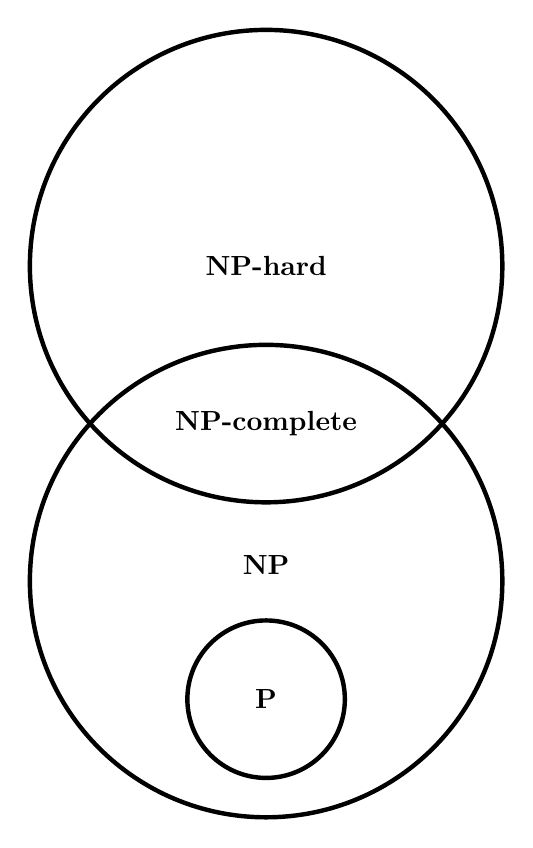
\begin{tikzpicture}
						\draw[ultra thick] (0,0) circle (3cm);
						\node at (current bounding box.center) {\textbf{NP-hard}};
						\draw[ultra thick] (0,-4) circle (3cm);
						\node at (current bounding box.center) {\textbf{NP-complete}};
						\node at ($(current bounding box.center) - (0, 1.8)$) {\textbf{NP}};
						\draw[ultra thick] (0,-5.5) circle(1cm);
						\node at ($(current bounding box.center) - (0, 3.5)$) {\textbf{P}};
					\end{tikzpicture}
					\caption{\centering Visualisation of the sets P, NP, NP-hard and NP-complete.}
					\label{fig:p,np,npcomplete}
				\end{figure}
				
				Since all problems in \textit{NP} can be reduced to any \textit{NP-complete} problem, if a deterministic polynomial time algorithm can be found for an \textit{NP-complete} problem, it would also mean that the set \textit{NP} is polynomial-time solvable, proving \textit{NP} and \textit{P} are equal sets. The question of whether \textit{P = NP} has famously been immortalised as one of the millennium prize problems from the Clay Institute of Mathematics \cite{claymathMillenniumPrize}.
				
%				why polynomial > exponential
				
				The reason polynomial-time algorithms are preferable is because these algorithms have time complexities bounded by $O(p(n))$, where $p$ is a polynomial function and $n$ is the input size \cite{computers-and-intractability}. Conversely, algorithms whose time complexity cannot be so bounded are deemed exponential-time algorithms \cite{computers-and-intractability}. The distinction between these two becomes more apparent as input sizes increase. Table \ref{tab:compare-2n-n2} illustrates why polynomial-time algorithms are preferred over exponential-time algorithms.
				
				\begin{table}
					\caption{\centering Comparison between (polynomial) $n^2$ algorithm and (exponential) $2^n$ algorithm as input size, $n$ increases}
					\label{tab:compare-2n-n2}
					\begin{center}
						\begin{tabularx}{\linewidth}{|c|*{6}{>{\centering\arraybackslash}X|}}
							\hline
							\multirow{2}{*}{\textbf{Time Complexity}} & \multicolumn{6}{c|}{\textbf{$n$}}\\ \cline{2-7}
							 & \multicolumn{1}{c|}{\textbf{10}} & \multicolumn{1}{c|}{\textbf{20}} & \multicolumn{1}{c|}{\textbf{30}} & \multicolumn{1}{c|}{\textbf{40}} & \multicolumn{1}{c|}{\textbf{50}} & \multicolumn{1}{c|}{\textbf{60}} \\
							\hline
							\textit{$n^2$} & .0001\newline seconds & .0004\newline seconds & .0009\newline seconds & .0016\newline seconds & .0025\newline seconds & .0036\newline seconds \\
							\hline
							\textit{$2^n$} & .001\newline seconds & 1.0\newline seconds & 17.9\newline minutes & 12.7\newline days & 35.7\newline years & 366\newline centuries \\
							\hline
						\end{tabularx}
					\end{center}
				\end{table}
				
			\subsection{Understanding the Proof}\label{subsec:understanding-proof}
			
				There are two necessary steps to be taken in order to prove that a problem, $X$ is \textit{NP-complete} \cite{npcompleteness}:
				
				\begin{enumerate}
					\item Show that $X \in $ \textit{NP} by finding a nondeterministic algorithm or giving a polynomial-time verifying algorithm.
					\item Show that $X \in$ \textit{NP-complete} by reducing a known \textit{NP-complete} problem to $X$. This is sufficient since problems in \textit{NP-complete} are also inherently \textit{NP-hard}.
				\end{enumerate} 

%				REDUCTIONS
				In the context of complexity theory, reductions are polynomial-time algorithms that convert inputs of one problem into equivalent inputs of another \cite{npcompleteness}. Reductions are useful when proving \textit{NP-completeness} \cite{cc:modern}. This is because a reduction from one problem to another implies that the latter is at least as hard as the former \cite{cc:modern}.
				
				Let $A$ and $B$ be two different problems. If $A$ is polynomial-time reducible to $B$, the following are true \cite{npcompleteness}:
				
				\begin{itemize}
					\item $B \in $ \textit{P} $\implies$ $A \in $ \textit{P}
					\item $B \in $ \textit{NP} $\implies$ $A \in $ \textit{NP}
					\item $A \in $ \textit{NP-hard} $\implies$ $B \in$ \textit{NP-hard}
				\end{itemize}
				
				\citeauthor{tetris-is-hard-even-to-approx} proved that optimising the following natural objective functions for Tetris is NP-complete \cite{tetris-is-hard-even-to-approx}:
				
				\begin{enumerate}
					\item maximising the number of rows cleared;
					\item maximising the number of pieces placed;
					\item maximising the number of Tetrises;
					\item minimising the height of the stack.
				\end{enumerate}
				
				Given a deterministic, finite piece sequence, \citeauthor{tetris-is-hard-even-to-approx} proposed that these objectives are in \textit{NP} by demonstrating an algorithm that  guesses a sequence of piece placements and verifies the legality and achievement of the objective in polynomial time \cite{tetris-is-hard-even-to-approx}. The legality of a piece placement, more specifically its rotation, can be checked in constant time since checking whether a rotation is legal looks only at the immediate space neighbouring the Tetrimino \cite{tetris-is-hard-even-to-approx}. Verifying if these objectives are met can be done in some time poly($|G|$), where $G$ represents the initial board state and the piece sequences of a game, $\langle G = B_0, P_1, ... , P_p \rangle$ \cite{tetris-is-hard-even-to-approx}.
				
				To prove that these objectives were NP-hard, the authors reduced the 3-PARTITION problem, a known NP-complete problem, to the natural objectives of Tetris \cite{tetris-is-hard-even-to-approx}. The 3-PARTITION problem is defined as follows \cite{tetris-is-hard-even-to-approx}:
				
				\noindent \textbf{Given:} A sequence $a_1,...,a_3s$ of non-negative integers and a non-negative integer $T$, so that $T/4 < a_i < T/2$ for all $1 \le i \le 3s$ and so that $\sum_{i=1}^{3s}a_i = sT$.
				
				\noindent \textbf{Output}: Can $\{a_1,...,a_3s\}$ be partitioned into $s$ disjoint subsets $A_1,...,A_s$ so that for all $1 \le j \le s$, we have $\sum_{a_i \in A_j}a_i = T$?
				
				With special initial matrices, \citeauthor{tetris-is-hard-even-to-approx} were able to prove that instances of 3-PARTITION can be mapped to instances of the 4 objective functions \cite{tetris-is-hard-even-to-approx}. In \citeyear{tetris-o1-np-hard}, \citeauthor{tetris-o1-np-hard} also proved that Tetris is NP-hard even when restricted to constant-sized rows or columns \cite{tetris-o1-np-hard}.
			
		\section{Addressing NP-complete Problems}
		
			% Explain the different approaches taken to solving NP-complete problems, more specfically on Tetris
			
			
		
		\section{Nature-inspired Algorithms}
		
			% Explain reasoning behind choosing nature-inspired algorithms, nature-inspired for tetris
		
		\section{Playing Tetris with Nature-inspired Algorithms}
		
			% Show examples of other work that has attempted to play Tetris with NIA
		
		\section{Identifying the Research Gaps}
		
			% No Versus
		
		\section{Concluding the Review}
	
	\chapter{Technical Plan}
	
		% Graphical and textual description is provided for flow of information between components in the system/stages in the research study.
		% Graphical overview of system/research study corresponds to the textual description provided with no errors.	
		%Excellent description is provided for all methodologies, tools and techniques used to specify, design, build, test, integrate, document and deliver work products throughout the project along with the relevant supporting documents.
		% All documents provided are well-drawn/well-written, complete and correct. The purpose and role of each document in the project is stated clearly.
		
		% Defining rules
	
	\chapter{Work Plan}
		
		% Excellent description of all work activities to be performed during the project, relationship among the activities and the resultant work products for each activity.
		% Scheduled duration for each work activity is justified and supported by the identified project risk factors and work decomposition that each activity requires.
		% The whole project schedule, milestones and activitiy lists are depicted professionally on the Gantt chart with all dependencies, predecessor and successor work activities denoted clearly.
	
	\printbibliography[heading={bibnumbered}, title={References}]
		
\end{document}